% move all configuration stuff into one file so we can focus on the content
\documentclass[aspectratio=169,hyperref={pdfpagelabels=false,colorlinks=true,linkcolor=white,urlcolor=lightblue},xcolor={table},t]{beamer}

%%%%%%%%%%%%%%%%%%%%%%%%%%%%%%%%%%%%%%%%%%%%%%%%%%%%%%%%%%%%%%%%%%%%%%%%%%%%%%%%%%
%%%%%%%%%%%%%%%%%%%%%%%%%%%%%%%%%%%%%%%%%%%%%%%%%%%%%%%%%%%%%%%%%%%%%%%%%%%%%%%%%%
% packages
\usepackage{pict2e}
\usepackage{epic}
\usepackage{amsmath,amsfonts,amssymb}
\usepackage{units}
\usepackage{fancybox}
\usepackage[absolute,overlay]{textpos} 
%\usepackage[table]{xcolor}
\usepackage{animate}
\usepackage{gensymb}
%\usepackage{graphicx}
%\usepackage{longtable}
\usepackage{multirow}
\usepackage{silence}
\usepackage{tikz}
\usepackage[backend=bibtex,style=ieee]{biblatex}
\AtEveryCitekey{\iffootnote{\tiny}{}}
%\addbibresource{include/references}



% fontsize
\let\Tiny=\tiny

%%%%%%%%%%%%%%%%%%%%%%%%%%%%%%%%%%%%%%%%%%%%%%%%%%%%%%%%%%%%%%%%%%%%%%%%%%%%%%%%%%
%%%%%%%%%%%%%%%%%%%%%%%%%%%%%%%%%%%%%%%%%%%%%%%%%%%%%%%%%%%%%%%%%%%%%%%%%%%%%%%%%%
% warnings
\pdfsuppresswarningpagegroup=1
\WarningFilter{biblatex}{Patching footnotes failed}
\WarningFilter{latexfont}{Font shape}
\WarningFilter{latexfont}{Some font shapes}
\WarningFilter{gensymb}{Not defining}


%%%%%%%%%%%%%%%%%%%%%%%%%%%%%%%%%%%%%%%%%%%%%%%%%%%%%%%%%%%%%%%%%%%%%%%%%%%%%%%%%%
%%%%%%%%%%%%%%%%%%%%%%%%%%%%%%%%%%%%%%%%%%%%%%%%%%%%%%%%%%%%%%%%%%%%%%%%%%%%%%%%%%
% theme & layout
\usetheme{Frankfurt}
\useinnertheme{rectangles}


%%%%%%%%%%%%%%%%%%%%%%%%%%%%%%%%%%%%%%%%%%%%%%%%%%%%%%%%%%%%%%%%%%%%%%%%%%%%%%%%%%
\setbeamertemplate{frametitle}[default][colsep=-4bp,rounded=false,shadow=false]
\setbeamertemplate{frametitle}
{%
    \nointerlineskip%
    %\vskip-0.5ex
    \begin{beamercolorbox}[wd=\paperwidth,ht=3.5ex,dp=0.6ex]{frametitle}
        \hspace*{1.3ex}\insertframetitle%
        
        \hspace*{1.3ex}\small\insertframesubtitle%
    \end{beamercolorbox}%
    \begin{textblock*}{100mm}(13.75cm,1cm)
        
\includegraphics[height=.4cm,keepaspectratio]{../shared/Logo_GTCMT_white}
    \end{textblock*}
}


%%%%%%%%%%%%%%%%%%%%%%%%%%%%%%%%%%%%%%%%%%%%%%%%%%%%%%%%%%%%%%%%%%%%%%%%%%%%%%%%%%
\setbeamertemplate{title page}[default][colsep=-4bp,rounded=false,shadow=false]
\setbeamertemplate{title page}
{
    %\begin{textblock*}{100mm}(15cm,.51cm)
            %\href{https://github.com/alexanderlerch/ACA-Slides/blob/2nd_edition/\jobname.pdf}{\includegraphics[height=.5cm,keepaspectratio]{graph/Logo_github}}\hspace*{2ex}
    %\end{textblock*}
    %\begin{textblock*}{100mm}(15cm,1.3cm)
            %\href{\IEEELink}{\includegraphics[height=.5cm,keepaspectratio]{graph/icon/book}}\hspace*{2ex}
    %\end{textblock*}
    \vskip-10ex
    \begin{beamercolorbox}[wd=\paperwidth,ht=.7\paperheight,dp=0.6ex]{frametitle} %35ex
        %\begin{flushright}
            %\href{http://www.gtcmt.gatech.edu}{
\includegraphics[height=.8cm,keepaspectratio]{graph/Logo_GTCMT_black}}\hspace*{2ex}
        %\end{flushright}
        
        \hspace*{1.8ex}\LARGE\inserttitle%
        
        \vspace*{.5ex}
        
        \hspace*{1.3ex}\small\insertsubtitle%
        
        \vspace*{.5ex}
    \end{beamercolorbox}%
    \nointerlineskip%
    \begin{beamercolorbox}[wd=\paperwidth,ht=.4\paperheight,dp=0.6ex]{page number in head/foot}
        %\vspace*{-.5ex}
        \hspace*{1.7ex}\small\insertauthor%
        
        %\hspace*{1.7ex}\small }%
        
        \vspace*{12ex}
        \vfill
        \begin{flushright}
            \href{http://www.gtcmt.gatech.edu}{
\includegraphics[height=.5cm,keepaspectratio]{../shared/Logo_GTCMT_black}}\hspace*{2ex}
        \end{flushright}
    \end{beamercolorbox}%
}


%%%%%%%%%%%%%%%%%%%%%%%%%%%%%%%%%%%%%%%%%%%%%%%%%%%%%%%%%%%%%%%%%%%%%%%%%%%%%%%%%%
%\makeatother
\setbeamertemplate{footline}
{
  \leavevmode%
  \hbox{%
  \begin{beamercolorbox}[wd=.5\paperwidth,ht=2.25ex,dp=1ex,left,leftskip=1ex]{page number in head/foot}%
    \insertsubtitle
  \end{beamercolorbox}%
  \begin{beamercolorbox}[wd=.5\paperwidth,ht=2.25ex,dp=1ex,right,rightskip=1ex]{page number in head/foot}%
    \hfill
    \insertframenumber{} / \inserttotalframenumber
  \end{beamercolorbox}}%
  \vskip0pt%
}
%\makeatletter


%%%%%%%%%%%%%%%%%%%%%%%%%%%%%%%%%%%%%%%%%%%%%%%%%%%%%%%%%%%%%%%%%%%%%%%%%%%%%%%%%%
\beamertemplatenavigationsymbolsempty
\setbeamertemplate{navigation symbols}{}
\setbeamertemplate{blocks}[default]%[rounded=false,shadow=false]
\setbeamertemplate{itemize item}[square]
\setbeamertemplate{itemize subitem}[circle]
\setbeamertemplate{itemize subsubitem}[triangle]
\setbeamertemplate{enumerate item}[square]
\setbeamertemplate{enumerate subitem}[circle]
\setbeamertemplate{enumerate subsubitem}[circle]


%%%%%%%%%%%%%%%%%%%%%%%%%%%%%%%%%%%%%%%%%%%%%%%%%%%%%%%%%%%%%%%%%%%%%%%%%%%%%%%%%%
% colors
\setbeamercolor{structure}{fg=darkgray}
\setbeamercovered{transparent} %invisible
\setbeamercolor{bibliography entry author}{fg=black}
\setbeamercolor*{bibliography entry title}{fg=black}
\setbeamercolor*{bibliography entry note}{fg=black}
\setbeamercolor{frametitle}{fg=black}
\setbeamercolor{title}{fg=white}
\setbeamercolor{subtitle}{fg=white}
\setbeamercolor{frametitle}{fg=white}
\setbeamercolor{framesubtitle}{fg=white}
\setbeamercolor{mini frame}{fg=white, bg=black}
\setbeamercolor{section in head/foot}{fg=white, bg=darkgray}
\setbeamercolor{page number in head/foot}{fg=black, bg=gtgold}
\setbeamercolor{item projected}{fg=white, bg=black}

%---------------------------------------------------------------------------------

%%%%%%%%%%%%%%%%%%%%%%%%%%%%%%%%%%%%%%%%%%%%%%%%%%%%%%%%%%%%%%%%%%%%%%%%%%%%%%%%%%
%%%%%%%%%%%%%%%%%%%%%%%%%%%%%%%%%%%%%%%%%%%%%%%%%%%%%%%%%%%%%%%%%%%%%%%%%%%%%%%%%%
% title information
\title[]{MUSI6202: Digital Signal Processing for Music}   
\author[alexander lerch]{alexander lerch} 
%\institute{~}
%\date[Alexander Lerch]{}
%\titlegraphic{\vspace{-16mm}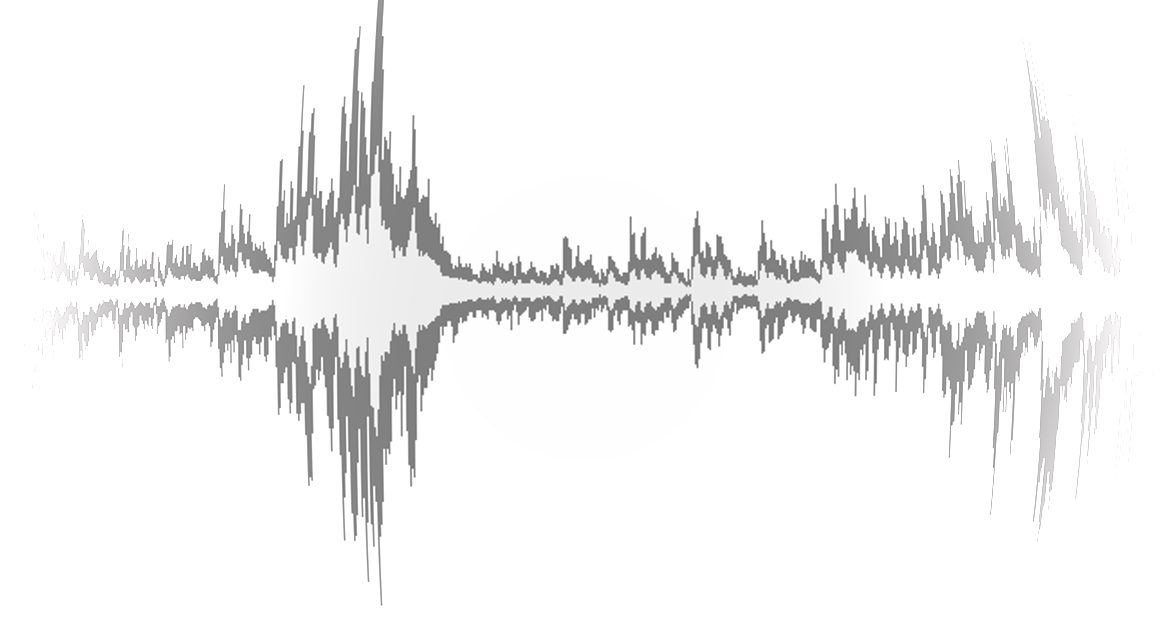
\includegraphics[width=\textwidth,height=3cm]{title}}

%%%%%%%%%%%%%%%%%%%%%%%%%%%%%%%%%%%%%%%%%%%%%%%%%%%%%%%%%%%%%%%%%%%%%%%%%%%%%%%%%%
%%%%%%%%%%%%%%%%%%%%%%%%%%%%%%%%%%%%%%%%%%%%%%%%%%%%%%%%%%%%%%%%%%%%%%%%%%%%%%%%%%
% colors
\definecolor{gtgold}{rgb}{.914, .664, 0} %0e7eed {rgb}{0.88,0.66,1,0.06} [234, 170, 0]/256 %96caff
\definecolor{darkgray}{rgb}{.15, .15, .15}
\definecolor{lightblue}{HTML}{0e7eed}
\definecolor{highlight}{rgb}{0, 0, 1} %_less!40

%%%%%%%%%%%%%%%%%%%%%%%%%%%%%%%%%%%%%%%%%%%%%%%%%%%%%%%%%%%%%%%%%%%%%%%%%%%%%%%%%%
%%%%%%%%%%%%%%%%%%%%%%%%%%%%%%%%%%%%%%%%%%%%%%%%%%%%%%%%%%%%%%%%%%%%%%%%%%%%%%%%%%
% relative paths
\graphicspath{{../graph/}}


%%%%%%%%%%%%%%%%%%%%%%%%%%%%%%%%%%%%%%%%%%%%%%%%%%%%%%%%%%%%%%%%%%%%%%%%%%%%%%%%%%
%%%%%%%%%%%%%%%%%%%%%%%%%%%%%%%%%%%%%%%%%%%%%%%%%%%%%%%%%%%%%%%%%%%%%%%%%%%%%%%%%%
% units
\setlength{\unitlength}{1mm}

%%%%%%%%%%%%%%%%%%%%%%%%%%%%%%%%%%%%%%%%%%%%%%%%%%%%%%%%%%%%%%%%%%%%%%%%%%%%%%%%%%
%%%%%%%%%%%%%%%%%%%%%%%%%%%%%%%%%%%%%%%%%%%%%%%%%%%%%%%%%%%%%%%%%%%%%%%%%%%%%%%%%%
% math
\DeclareMathOperator*{\argmax}{argmax}
\DeclareMathOperator*{\argmin}{argmin}
\DeclareMathOperator*{\atan}{atan}
\DeclareMathOperator*{\arcsinh}{arcsinh}
\DeclareMathOperator*{\sign}{sign}
\DeclareMathOperator*{\tcdf}{tcdf}
\DeclareMathOperator*{\si}{sinc}
\DeclareMathOperator*{\princarg}{princarg}
\DeclareMathOperator*{\arccosh}{arccosh}
\DeclareMathOperator*{\hwr}{HWR}
\DeclareMathOperator*{\flip}{flip}
\DeclareMathOperator*{\sinc}{sinc}
\DeclareMathOperator*{\floor}{floor}
\newcommand{\e}{{e}}
\newcommand{\jom}{\mathrm{j}\omega}
\newcommand{\jOm}{\mathrm{j}\Omega}
\newcommand   {\mat}[1]    		{\boldsymbol{\uppercase{#1}}}		%bold
\renewcommand {\vec}[1]    		{\boldsymbol{\lowercase{#1}}}		%bold

%%%%%%%%%%%%%%%%%%%%%%%%%%%%%%%%%%%%%%%%%%%%%%%%%%%%%%%%%%%%%%%%%%%%%%%%%%%%%%%%%%
%%%%%%%%%%%%%%%%%%%%%%%%%%%%%%%%%%%%%%%%%%%%%%%%%%%%%%%%%%%%%%%%%%%%%%%%%%%%%%%%%%
% media9
\newcommand{\includeaudio}[1]{
\href{run:audio/#1.mp3}{
\includegraphics[width=5mm, height=5mm]{graph/SpeakerIcon}}}

\newcommand{\includeanimation}[4]{{\begin{center}
                        \animategraphics[autoplay,loop,scale=.7]{#4}{animation/#1-}{#2}{#3}        
                        \end{center}
                        \addreference{matlab source: \href{https://github.com/alexanderlerch/ACA-Plots/blob/master/matlab/animate#1.m}{matlab/animate#1.m}}}
                        \inserticon{video}}
                        
%%%%%%%%%%%%%%%%%%%%%%%%%%%%%%%%%%%%%%%%%%%%%%%%%%%%%%%%%%%%%%%%%%%%%%%%%%%%%%%%%%
%%%%%%%%%%%%%%%%%%%%%%%%%%%%%%%%%%%%%%%%%%%%%%%%%%%%%%%%%%%%%%%%%%%%%%%%%%%%%%%%%%
% other commands
\newcommand{\question}[1]{%\vspace{-4mm}
                          \setbeamercovered{invisible}
                          \begin{columns}[T]
                            \column{.9\textwidth}
                                \textbf{#1}
                            \column{.1\textwidth}
                                \vspace{-8mm}
                                \begin{flushright}
                                     
\includegraphics[width=.9\columnwidth]{graph/question_mark}
                                \end{flushright}
                                \vspace{6mm}
                          \end{columns}\pause\vspace{-12mm}}

\newcommand{\toremember}[1]{
                        \inserticon{lightbulb}
                        }

\newcommand{\matlabexercise}[1]{%\vspace{-4mm}
                          \setbeamercovered{invisible}
                          \begin{columns}[T]
                            \column{.8\textwidth}
                                \textbf{matlab exercise}: #1
                            \column{.2\textwidth}
                                \begin{flushright}
                                     \includegraphics[scale=.5]{graph/logo_matlab}
                                \end{flushright}
                                %\vspace{6mm}
                          \end{columns}}

\newcommand{\addreference}[1]{  
                  
                    \begin{textblock*}{\baselineskip }(.98\paperwidth,.5\textheight) %(1.15\textwidth,.4\textheight)
                         \begin{minipage}[b][.5\paperheight][b]{1cm}%
                            \vfill%
                             \rotatebox{90}{\tiny {#1}}
                        \end{minipage}
                   \end{textblock*}
                    }
                    
\newcommand{\figwithmatlab}[1]{
                    \begin{figure}
                        \centering
                        \includegraphics[scale=.7]{#1}
                        %\label{fig:#1}
                    \end{figure}
                    
                    \addreference{matlab source: \href{https://github.com/alexanderlerch/MUSI-6202/blob/main/matlab/plot#1.m}{plot#1.m}}}
\newcommand{\figwithref}[2]{
                    \begin{figure}
                        \centering
                        \includegraphics[scale=.7]{#1}
                        \label{fig:#1}
                    \end{figure}
                    
                    \addreference{#2}}  
                                    
\newcommand{\inserticon}[1]{
                    \begin{textblock*}{100mm}(14.5cm,7.5cm)
                        \includegraphics[height=.8cm,keepaspectratio]{graph/#1}
                    \end{textblock*}}            

%%%%%%%%%%%%%%%%%%%%%%%%%%%%%%%%%%%%%%%%%%%%%%%%%%%%%%%%%%%%%%%%%%%%%%%%%%%%%%%%%%
%%%%%%%%%%%%%%%%%%%%%%%%%%%%%%%%%%%%%%%%%%%%%%%%%%%%%%%%%%%%%%%%%%%%%%%%%%%%%%%%%%
% counters
\newcounter{i}
\newcounter{j}
\newcounter{iXOffset}
\newcounter{iYOffset}
\newcounter{iXBlockSize}
\newcounter{iYBlockSize}
\newcounter{iYBlockSizeDiv2}
\newcounter{iXBlockSizeDiv2}
\newcounter{iDistance}

\newcommand{\IEEELink}{https://ieeexplore.ieee.org/servlet/opac?bknumber=9965970}

\addbibresource{../shared/references}



\subtitle{Part 2: Introduction}

%%%%%%%%%%%%%%%%%%%%%%%%%%%%%%%%%%%%%%%%%%%%%%%%%%%%%%%%%%%%%%%%%%%%%%%%%%%%
\begin{document}
    % generate title page
	\title[]{Digital Signal Processing for Music}   
\author[alexander lerch]{alexander lerch} 
%\institute{~}
%\date[Alexander Lerch]{}
\titlegraphic{\vspace{-16mm}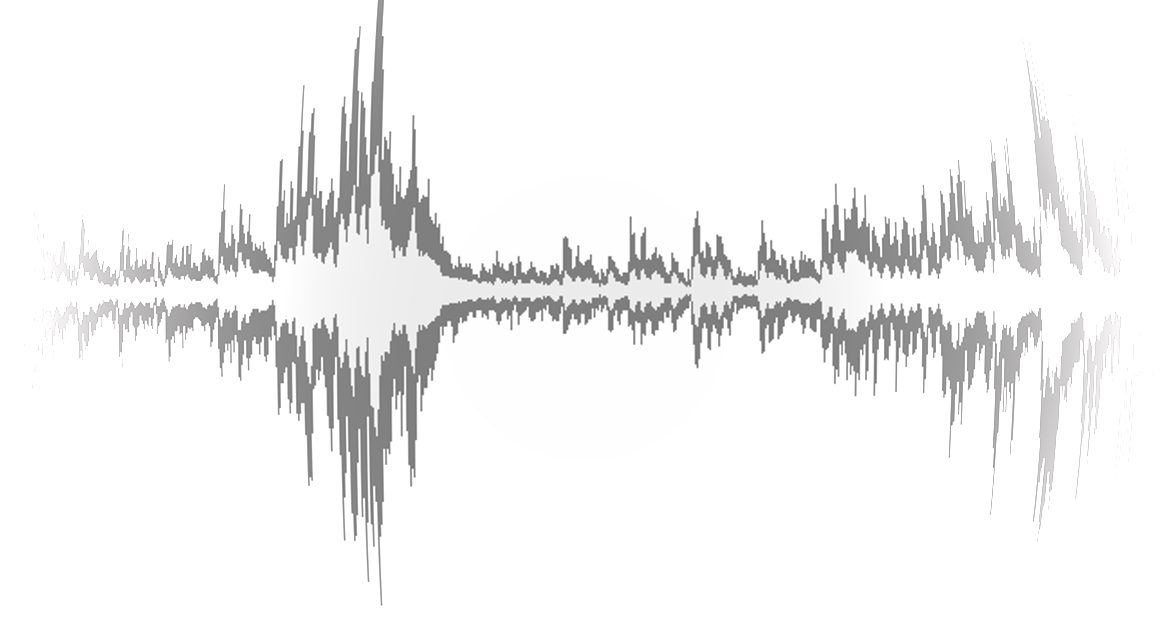
\includegraphics[width=\textwidth,height=3cm]{title}}


\begin{frame}
    \titlepage
    %\vspace{-5mm}
    \begin{flushright}
        \href{http://www.gtcmt.gatech.edu}{
\includegraphics[height=.8cm,keepaspectratio]{../shared/Logo_GTCMT_black}}
    \end{flushright}
\end{frame}


\section{introduction}
\begin{frame}{introduction}{digital technology}
    \begin{itemize}
        \item   examples of everyday digital (audio) technology
            \begin{itemize}
                \item   \textbf{music listening}:
                    \begin{itemize}
                        \item   audio compression
                        \item   audio storage and streaming
                        \item   equalization and loudness adaptation
                        \item   \ldots
                    \end{itemize}
                \smallskip
                \item   \textbf{music production and synthesis}
                    \begin{itemize}
                        \item   recording and editing
                        \item   effects
                        \item   denoising
                    \end{itemize}
                \smallskip
                \item   \textbf{human computer interaction}
                    \begin{itemize}
                        \item   speech recognition
                        \item   text-to-speech
                    \end{itemize}
                \smallskip
                \item   \ldots
            \end{itemize}
    \end{itemize}
\end{frame}

\section{history}
\begin{frame}\frametitle{introduction}\framesubtitle{release of digital technology --- production}
    \vspace{-5mm}
	\begin{columns}
		\column{5cm}
			\begin{scriptsize}
			\begin{table}
					\begin{tabular}{lr}
					\hline
						\textbf{Product} & \textbf{Year} \\
					\hline%
					\uncover<1->{%
						\textbf{Sound Synthesis} &            \\
						
						NED Synclavier Synthesizer/Sampler &       1979 \\
						
						Fairlight CMI Synthesizer/Sampler &       1979 \\
						
						Linn LM-1 Drumcomputer/Sampler	&				1980	\\
						
						E-MU Emulator I Sampling Keyboard &       1981 \\
						
						\only<1>{\textcolor{gtgold}}{Yamaha DX-7 Syntheziser} &       1983\vspace{1mm}\\
						
					}%		
					\uncover<2->{%
						\textbf{Sound Processing/Effects} &            \\
						
						Lexicon Delta-T 101 Digital Delay & 1971 \\
						
						EMT 250 Digital Reverberation & 1976 \\
						
						\only<2>{\textcolor{gtgold}}{Lexicon L224 Digital Reverberation} &       1978\vspace{1mm} \\
							
					}%	
					\uncover<3->{%
						\textbf{Sound Editing} &            \\
						
						Sony DAE-1100 Digital Audio Editor &       1980 \\
						
						\only<3>{\textcolor{gtgold}}{Sony DAE-3000 Digital Audio Editor} &       1987 \\
		
						Sonic Solutions Harddisk Editing &       1988\vspace{1mm}\\
						
					}%
					\uncover<4->{%
						\textbf{Other} &            \\
						
						\only<4>{\textcolor{gtgold}}{MIDI Standard}	&			1983		\\
					\hline
					}
					\end{tabular}  
			\end{table}
			\end{scriptsize}
		\column{3cm}
			\only<1>{
				\begin{figure}
					\centering
					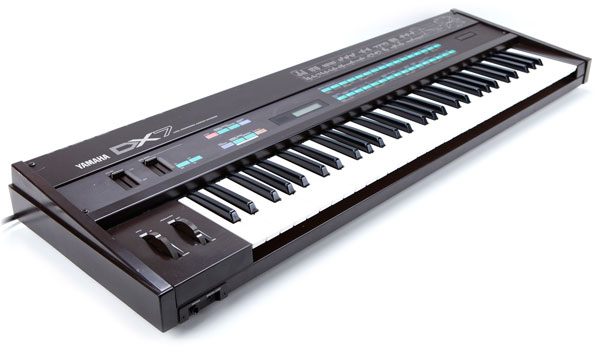
\includegraphics[scale=.3]{graph/yamaha_dx7}
				\end{figure}
			}
			\only<2>{
				\begin{figure}
					\centering
					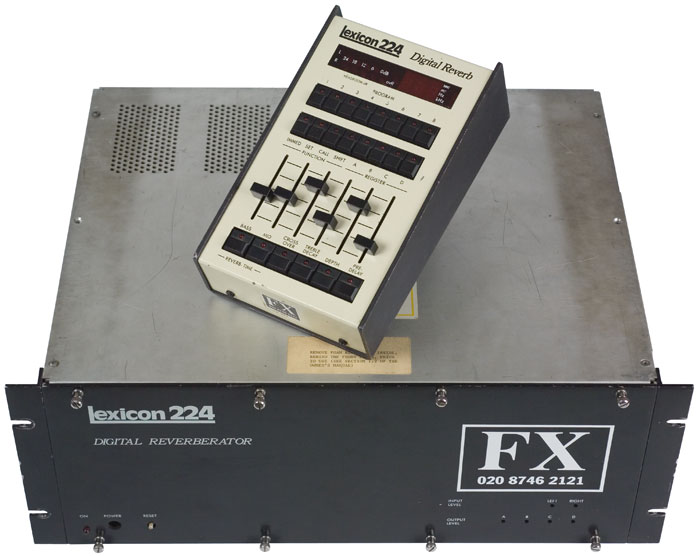
\includegraphics[scale=.15]{graph/lexicon224}
				\end{figure}
			}
			\only<3>{
				\begin{figure}
					\centering
					\includegraphics[scale=.4]{graph/sony_DAE3000}
				\end{figure}
			}
			\only<4>{
				\begin{figure}
					\flushright
					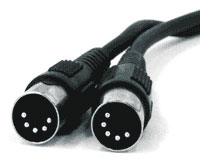
\includegraphics[scale=.76]{graph/midi_cable}
				\end{figure}
			}
	\end{columns}
\end{frame}

\begin{frame}\frametitle{introduction}\framesubtitle{release of digital technology --- storage \& consumer}
    \vspace{-5mm}
	\begin{columns}
		\column{5cm}
			\begin{scriptsize}
			\begin{table}
				\begin{tabular}{lr}
				\hline
					\textbf{Digital Storage} & \textbf{Year} \\
				\hline%
				\uncover<1->{%
					\textbf{Professional} &            \\
					PCM-1600 (U-matic)	&			1978	\\
					PCM-1 (Betamax)	&			1978	\\
					
					Digital Multitrack (3M, Sony)	&			1978	\\
					
					Alesis ADAT &       1991 \\
					
					\only<1>{\textcolor{gtgold}}{Tascam DA-88} &       1993\vspace{1mm}  \\
				}%
				\uncover<2->{%
					\textbf{Consumer} &            \\
					\only<2>{\textcolor{gtgold}}{Compact Disc} &       1982/83\\
					Digital Audio Tape (DAT) &       1987\\
					MiniDisc &       1991\\
					Digital Compact Cassette &       1992\\
					DVD-Video & 	1997\\
					DVD-Audio & 1999\\
					SACD & 1999\\
					\hline
				}
				\end{tabular}  
			\end{table}
			\end{scriptsize}
		\column{3cm}
			\only<1>{
				\begin{figure}
					\centering
					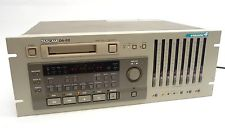
\includegraphics[scale=1.5]{graph/tascam_da88}
				\end{figure}
			}
			\only<2>{
				\begin{figure}
					\centering
					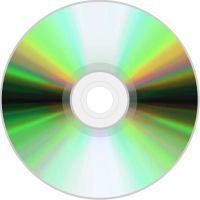
\includegraphics[scale=.3]{graph/compact_disc}
				\end{figure}
			}
	\end{columns}
\end{frame}


\begin{frame}{introduction}{reasons for digital equipment}
	\begin{itemize}
        \item   \textbf{storage}:
            \begin{itemize}
                \item   lossless copying and archiving of digital content
            \end{itemize}
        \smallskip
        \item<2->   \textbf{editing \& processing} 
            \begin{itemize}
                \item   splicing of recordings
                \item   fast convolution
                \item   granular processing/time-stretching/pitch-shifting
            \end{itemize}
        \smallskip
		\item<3->	\textbf{technical characteristics}
			\begin{itemize}
				\item	SNR, distortion, transfer functions, ...
			\end{itemize}
        \bigskip
        \item<4->   \textbf{dropping prices} for digital hardware and software (compared to analogue equipment)
    \end{itemize}
\end{frame}

\section{current trends}
\begin{frame}{introduction}{current trends \& developments}
	\begin{itemize}
		\item	\textbf{resolution and data rates}
			\begin{itemize}
				%\item	higher bit resolution and sample rates?
				\item	lower data rates for compression formats
			\end{itemize}
		\smallskip
        \item<2->   \textbf{audio formats}
			\begin{itemize}
				\item	multichannel \& WFS, 3D acoustics in general
                \item   object-based audio
			\end{itemize}
		%\pause
		%\item	\textbf{further digitization and improvements of equipment}
			%\begin{itemize}
				%\item	microphones \& speakers
				%\item	(remote control of) DSP-enabled systems
				%\item	converters \& storage
			%\end{itemize}
		%\pause
		%\item	\textbf{transmission and distribution channels}
			%\begin{itemize}
				%\item	streaming on demand
				%\item	subscription models
			%\end{itemize}
		\smallskip
        \item<3->   \textbf{production environments}
			\begin{itemize}
				\item	online collaboration/musicianship
                \item   machine musicianship
			\end{itemize}
		\smallskip
        \item<4->   \textbf{software}
			\begin{itemize}
				\item	machine listening:  music recommendation systems, etc.
				\item	signal- and user-adaptive audio production software
				\item	computer-aided editing, composition, and performance systems
                \item   interactive and creative audio consumer software
			\end{itemize}
	\end{itemize}
\end{frame}
\section{class content}
\begin{frame}{introduction}{relation to class context}
	\begin{itemize}
		\item	in this class, we will learn the basics of
            \begin{itemize}
                \item   \textbf{digitizing} an analogue signal
                \smallskip
                \item   \textbf{transforming and analyzing} a digital signal
                \smallskip
                \item   \textbf{processing} a digital signal
                \smallskip
                \item   \textbf{applying standard effects} to a digital signal
                \smallskip
                \item   \textbf{encoding and decoding} a digital signal
            \end{itemize}
	\end{itemize}
\end{frame}


\end{document}

